\documentclass{scrreprt}
\usepackage[utf8]{inputenc}

\usepackage{natbib}
\usepackage{graphicx}
\usepackage{tikz}
\usepackage{pgfplots}
\pgfplotsset{compat=1.12}
\usepackage{textcomp}

\usepackage{amsmath} % Math
\usepackage{hyperref} % Hyperlinks
\usepackage[noabbrev]{cleveref} % Clickable hyperlinks
\usepackage[parfill]{parskip} % Remove intent on paragraph
\usepackage{caption} % add captions
\usepackage{url} % URLs
\usepackage{pdfpages} %add pdf as pages
\usepackage{glossaries} % for abbreviation list
\usepackage{subfig} % multiple images in one figure
\usepackage[labelfont=bf]{caption} 
%\usepackage[doublespacing]{setspace}
%\usepackage[nopostdot,style=super,nonumberlist,toc]{glossaries}

\renewcommand{\baselinestretch}{1.5}

% Edit the meta.tex file to change title and author names

\usepackage{tocbibind} % fix for wrong hyperlink for toc, tof and tot

\newcommand{\mytitle}{\textbf{A Control System for Autonomous Vehicles}\par
Forward and Inverse Kinematics}
\newcommand{\myauthor}{Stefan Bui}
\newcommand{\mysupervisor}{Sven Fjeldass}

\title{\mytitle}
\author{\myauthor}
\date{\today}

% Source of figures
\newcommand*{\captionsource}[1]{
    \fontsize{7}{6}\selectfont{
        \hspace{\linewidth}
        \textbf{Source:} #1
    }
}

% Fix stuff with glossary and koma-script
\AtBeginDocument{%
  \setlength{\glsdescwidth}{0.8\columnwidth}%
  \setlength{\glspagelistwidth}{.1\columnwidth}%
}

\newglossarystyle{custom_super}
{
    \setglossarystyle{long3colheader}%
    \renewcommand*{\glossaryheader}{}%  
    \renewcommand{\glossentry}[2]{%
        \textbf{\glsentryitem{##1}\glstarget{##1}{\glossentryname{##1}}}
        & \glossentrydesc{##1}
        & ##2
        \tabularnewline}%
}

\makeglossaries

\newglossaryentry{AUV}
{
        name=AUV,
        description={Autonomous underwater vehicle}
}

\newglossaryentry{End-effector}
{
        name=End-effector,
        description={The device at the end of a robotic arm}
}


\newglossaryentry{Basis}
{
        name=Basis,
        description={A set of unit vectors pointing in a space in a Cartesian coordinate system}
}

\newglossaryentry{TGroup}
{
        name=TGroup,
        description={A class in GeoMod that contains geometric data with designated coordinate frame eometric data with designated coordinate frame}
}

\newglossaryentry{Workspace}
{
        name=Workspace,
        description={The volume of space a robot's end-effector can reach, limited by its joints and presence of obstacles}
}


%----- DOCUMENT -----
\begin{document}

% The title page
\begin{titlepage}

\begin{center}
    
    ~\\[2.0cm]
    
    \Large \textbf{Semester project}\\[2.5cm]
     
    % Set the title of the Document between two horizontal lines
    \hrule
    {\LARGE \mytitle}	% print the title of the document
    \vspace{0.5cm}
    \hrule
    
    \vspace{1.0cm}
    
    \LARGE \textbf{\myauthor}\\[2.5cm]
    
    \Large supervised by\par
	\mysupervisor
    
    \vfill
    {\large \today}
    
    \vspace{1.0cm}
    
    
\includegraphics[height=1.5cm]{images/ntnu_logo.pdf}
    
\end{center}

%\large{Norwegian University of Science and Technology
%\\[0.2cm]
%Faculty of Engineering Science and Technology\\[0.2cm]
%Department of Engineering Design and Materials} 
%\vspace{1.5cm} 

\end{titlepage}

%Roman numbering
\pagenumbering{Roman}
\setcounter{page}{1}

\phantomsection
\addcontentsline{toc}{chapter}{Preface}
\vspace*{\fill}
{\centering\huge\bfseries Preface \par}
\noindent This project thesis was written in the fall 2016 for my specialisation project. The project with a specialisation course is a prerequisite before one can write a master thesis. Among many topics to write about, the subject of autonomous systems piqued my interest and was chosen for my assignment. The specialisation course, TMM4280 - Advanced Product Development, was taken alongside this project.

I would like to express my gratitude to my supervisor Professor Sven Fjeldaas for his first-rate guidance and helpful inputs throughout this project.

\vspace*{\fill}


\clearpage
\phantomsection
\addcontentsline{toc}{chapter}{Abstract}
\vspace*{\fill}
{\centering\huge\bfseries Abstract \par}

This paper blabla development of a unified control system for models and camera objects. three dimensional path, translation, orientaion, position, rotation, path as network. much of the physics are already implemented, but works independent. Goal to see how it all can colaborate together. software modules. qt framework for multiplatform



\vspace*{\fill}


\clearpage
%\addcontentsline{toc}{chapter}{Table of Contents}
\tableofcontents

\listoffigures
%\addcontentsline{toc}{chapter}{\listfigurename}

%\listoftables
%\addcontentsline{toc}{chapter}{\listtablename}

\glsaddall % make it possible to print glossary without references
\printglossary[title=Abbreviations,nonumberlist, style = custom_super] % print the glossary
\addcontentsline{toc}{chapter}{Abbreviations}

\clearpage
\pagenumbering{arabic}
\setcounter{page}{1}

% Main matter - edit corresponding file under content/ to change
\chapter{Introduction}

Robotics is commonly applied in industry to solve challenging tasks efficiently. One of the advantages of robotics lies in the fact that robots do not suffer from the same limitations as humans. Therefore, not only can robots perform many of the same tasks, but also tasks that seemingly would be physically impossible for a human being. An autonomous underwater vehicle (AUV) has traditionally been used for mapping and monitoring the ocean for military purposes. Today, its applications are frequently employed by the oil and gas industry, scientist and roboticists for commercial survey services. The advancements in technology has unlocked possibilities for complex missions, and improved the ability of the AUV to further interact with the surroundings. The degree of autonomy is based on how it gathers information of its environment, as well as how it adjusts and adapts to unpredicted variables.

This thesis will describe the development of a control system based on geometrical models and forward kinematics for vehicles and tools with a graphical user interface (GUI). To facilitate for an autonomous mode, an implementation of a reference system is desired for setting up and altering paths while the software is in continuous operation.
Existing functionality regarding forward and inverse kinematics, network of paths and a GUI will also be presented. The primary goal is to show how the system interacts with the developed functionality, and serve as a proof of concept on how operations between vehicle, tools and environment behave.

\section{Background}

The GeoMod project is an ongoing project that has been in development for more than ten years. The project was initiated to explore the vast applications that autonomous vehicles could offer, and is meant to be a learning and development platform for students. The principal aim for this project encompasses interesting issues concerning many types of vehicles. Over the years, changes and requirements have been altered to keep up with new technologies and software. In the present day, a prerequisite for GeoMod is to be a platform independent software and developed with the cross-platform application framework Qt. 

\section{Objectives}
\label{chap:objectives}

From the project assignment, also found in appendix A Project Assignment, the interpreted objectives can be broken down to the following sub-objectives:

\begin{itemize}
  \item Establish a control system based on forward kinematics for vehicles and tools.
  \item Enable geometric models to follow a freely chosen, an absolute or a given path.
  \item Enable inverse kinematics to regulate the relation between the manipulator and a chosen path.  
  \item Implement a GUI for the control system with consideration for autonomous mode used by other software.
\end{itemize}


\noindent These objectives are defined to further develop the software GeoMod. Furthermore, it is stated in the project description that the assignment is based on a geometric modelling that can control and visualise several models of freely movable joints and gliding mechanisms simultaneously. The described system is an overall control system for geometric and mathematical model type in GeoMod. It is desirable to have a system that enables the mechanism to handle tool to follow certain paths by forward and inverse kinematics. Paths are designed as networks with associated curves. The resulting position and orientation can be calculated with a method outlined by supervisor Professor Sven Fjeldaas. The ability for tools to follow a determined path was partially implemented by Martin Lygre Furevik in his master thesis from 2016 \cite{martin}. In consultant with the supervisor, the defined key goal of this assignment was to create an intelligible and a user-friendly GUI for the control system. The priority to establish an overall working comprehension of the system was set with regards to much functionality of the system already working independently.


\section{Approach}

The essential overall understanding and familiarity with the existing system of GeoMod was required before starting with the practical parts of the assignment, i.e. coding. The associated functionalities that have been developed in the earlier phases of the project was needed to be comprehended. Many of the functions resolving some of the objectives already existed, but was implemented and hard-coded to work independently for testing and demonstration of a distinct solution. After getting known with the software and acquiring a clearly understanding of how it works, the implementation of a control system could begin. 

The control system is based on predefined geometrical models in GeoMod, made in earlier projects as a basis for testing. Parts of the existing library and modules required some minimal changes without affecting other parts of the software. Redesign was deemed necessary in some parts where consideration of graphical and functional areas of the software was not clearly defined.
\chapter{Existing Systems, Tools and Earlier work}

\section{Qt}

\section{GeoMod}

\section{Tools and Paths}

\section{Control System}



\chapter{Theory}
\label{chap:theory}

\section{Forward and Inverse Kinematic}

\subsection{Forward Kinematics}

Forward kinematics is about finding the position and orientation of the tool point, which is generally the robot end-effector, from the joint angles along the robot arm. The calculation is based on specified joint angles as parameters. The position is found by going forward from the base of the robot toward the end-effector. For robot using forward kinematics is not very practical. \cite{forward_kinematics}

\subsection{Inverse Kinematics}

The inverse kinematics is the opposite of the forward kinematics. This means inverse kinematics refers to what particular angles should be set for all the robot joints, in order for the end-effector to be in the desired position and orientation. This way of behaviour is more relevant to most real world applications and tasks performed by robots. \cite{inverse_kinematics}

One of the big differences between forward and inverse kinematics is that forward kinematics usually has one distinct solution. Setting all the angles of the joints for a robot arm to certain values, will generally result that the tool point will end in one particular position. However, inverse kinematics is quite different. Depending on the situation and design structure of the robot arm, there could be many ways to position the joints of a robot arm and angle them to reach a specific point in workspace. A good example of this would be to use your own arm to reach a point in space, from as many different possible ways you can position your shoulder, wrist or elbow joint. Inverse kinematics can yield multiple solutions, but that does not necessarily mean all solution is feasible. Each solution need to be validate against criteria given by the robot specifications and workspace. These solutions have to satisfy the constraints of each joint and valid movements in a reachable workspace.


\section{Frame of Reference}

\section{Software Architecture and Design Patterns}
\subsection{MVC}
\subsection{Observer Pattern}




\chapter{Control System}

The implementation process of a control system is focused on existing independently modules and underlying features in the software. The stepwise procedure for this assignment was to take on the challenge of understanding the different modules and fuse these modules to a more unified solution. A dedicated and intuitive GUI for the control system was wanted. The purpose is to provide a more overall impression of an autonomous system to simplify further aid to test and demonstrate future implementation.


\section{Earlier Design Choices}

In the previously work done by students, independent modules were designed to have a control interface that was just suitable for their implementation objectives. Therefore, the intention of the interfaces does not represent the final purpose of the modules. In the current version of GeoMod, some modules involve going through a sequence of associated modules for usage and testing. One finds again that all modules have their own control interface,  which can lead to multiple frames appearing on the monitor. It can, therefore, be difficult to keep track of each interface and simultaneously wasting monitor space. Again, the functionality of these modules could be limited because it was developed and tested independently.

\label{chap:example}
The panel seen in \Cref{fig:controlpanels} (left) is the main menu and the first frame that is displayed when running GeoMod. This panel shows a good example of how modules accessed through a GUI and how it looks like currently. Let us take an example of how the procedure in GeoMod for visualising and controlling a geometric model of a triangle. The first step is to run the software GeoMod. The main menu will then appear. Subsequently, clicking on the button labelled camera on the main menu, opens the viewport seen previously in \Cref{fig:viewport} and a corresponding GUI for camera control. All the models mention beforehand in \Cref{chap:model} will by default be rendered (over each other) on the viewport. To further move the triangle, one needs to go back to the main menu frame, and click on the button with the label triangle. Like many of the other models, a new panel corresponding to the chosen model appear. From the new the panel, clicking the move button opens up the control panel for translation and rotation of the triangle, like the one seen earlier on \Cref{fig:controlcube}.

\begin{figure}[ht]
    \centering
    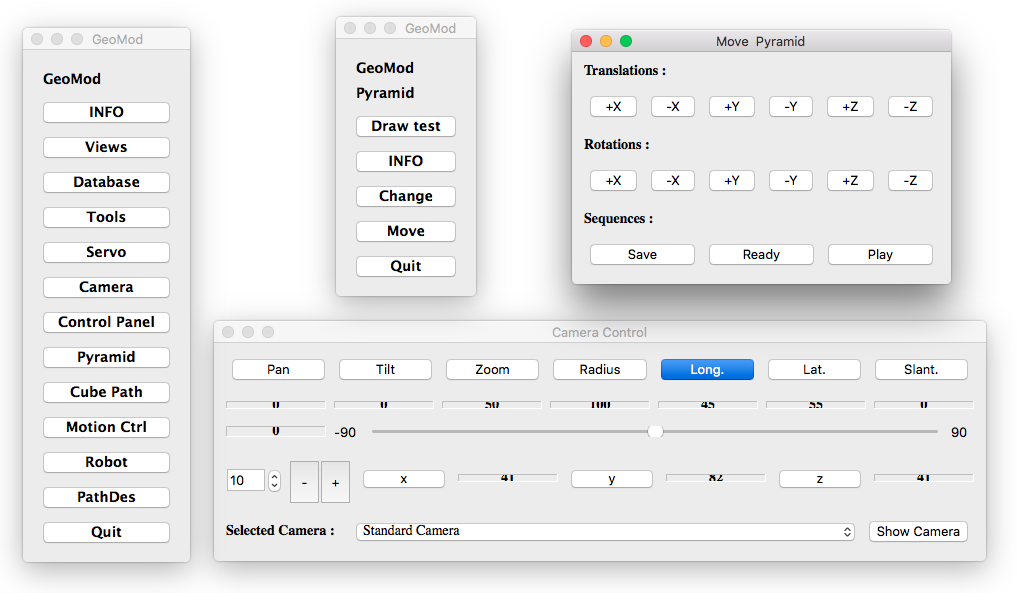
\includegraphics[height=8cm]{images/example_control.png}
    \caption[Control panels]{Left: Main Menu, top-middle: Model menu, top-right: Model control panel, bottom-right: Camera control panel}
    \label{fig:controlpanels}
\end{figure}

This example is meant to illustrate how messy and unintuitive this setup is, for something that should be somewhat straightforward to do. Notably, involving simultaneously control of multiple models would cause a headache. Not only is the main menu starting unnecessary long, but many of the buttons such as Pyramid and Cube Path are redundant as the graphical interfaces for those objects are the same. A clean up of redundancy and a structure for the graphical user interface is emphasised.

\section{Graphical User Interface}

In software development, the visual composition and behaviour of a graphical user interface is an essential part of the human-machine interaction. The GUI is meant to enhance the usability of the user and the underlying logical design of the software \cite{gui}. Qt simplifies much of the process of developing a GUI by providing graphical elements such as buttons, sliders, text, labels etc. These widgets are inherent from a class in Qt called QWidget \cite{qwidget}. In addition, Qt provides an easy way to structure widgets and communication between them. Qt's callback technique called Signal \& Slots, offers an automatic calling method produce from user interactions with widgets, which have been useful in the development of a graphical user interface \cite{signalslots}. The great thing about Qt, regarding GUI, is that it automatically uses the native graphical style (\Cref{fig:qstyle}) of the operating system it runs on. The advantage with a native theme is that users of the application do not need to get accustomed with a new design. They will be more comfortable with something they already know, as simplicity offers the best user experience of the functionality of an application. On the other hand, it is not guaranteed that the GUI is the same when ran on different operating systems. An example on this can be seen from camera control panel in \Cref{fig:controlpanels}, where the frame around the digits label is too small and narrow when ran on Mac operating system. That particular panel was implemented on a Linux operating system from a previously project. A customised design created primarily for the application can solve this uncertainty as all the operating systems are using the same theme style. Again, this requires a lot of time and works designing a theme from scratch as one also need to update the theme with new functionality added.

\begin{figure}[ht]
  \centering
  \subfloat[Windows]{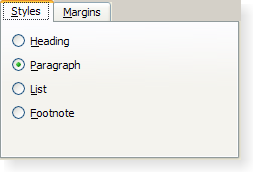
\includegraphics[width=0.3\textwidth]{images/windows.png}\label{fig:f1}}
  \hfill
  \subfloat[Linux]{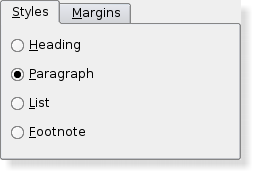
\includegraphics[width=0.3\textwidth]{images/linux.png}\label{fig:f2}}
  \hfill
  \subfloat[Mac]{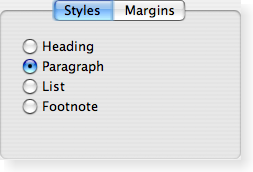
\includegraphics[width=0.3\textwidth]{images/mac.png}\label{fig:f3}}
  \caption[Natives operating system styles \cite{qstyle}]{Natives operating system styles \cite{qstyle}}
  \label{fig:qstyle}
\end{figure}


\section{Control Panel}

The objectives of the assignment (\Cref{chap:objectives}) explicitly tells to establish a control system for vehicles and tools. Thus the focused will be to adopt and utilise much of the implemented mechanics regarding the transformation control. By developing an overall control system, an arrangement of all future applicable functions have to be taken into consideration as best as possible. The GUI will be developed under the macOS operating system corresponding with macOS natives theme style.

Before implementing the control system, two main concerns needs to be thought about. What do we wish to govern? What areas of needs occurs? To the first question, the assignment emphasised on model and path control with the use of forward and inverse kinematics. In this project, an emergence of interest for the camera control arise. Like models and paths, the virtual camera consists of a basis related to the world space.  But unlike models and paths, cameras are moved in spherical coordinates that suit for its purpose. It is beforehand implemented a control panel for the camera with options to add more cameras and change viewport to a specific view of interest. Hence, this was taken into consideration for the implementation of the control system. Note that even if the camera control was relevant for the control system, an implementation of its usage was not the priority as it was outside the scope of the given assignment. However, the implemented GUI for the control system can also be applied to the cameras in future development. For the second question, it is important to know the intentions and usage of the various functions of the users. With that in mind, a graphical user interface can develop to fit the use of the users. Another important factor when designing a GUI is how organised and structured it is, to get sufficient overview of the system. As probably understood from the example in \Cref{chap:example}, overflow of framess and senseless procedure makes it complicated and clueless on how the system works.

\begin{figure}[ht]
    \centering
    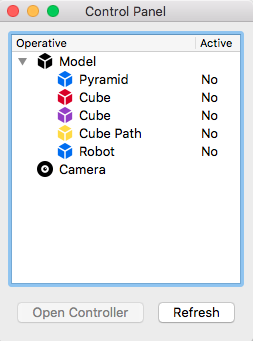
\includegraphics[height=6cm]{images/control_overview.png}
    \caption[Control overview panel]{Control overview panel}
    \label{fig:ctroverview}
\end{figure}

The idea behind the new design of the GUI was that each object should have its own control frame based on the same GUI. This approach makes it flexible to manage various types of objects simultaneously. As this method could result in an abundance of frames covering the monitor, a GUI with the overview of objects was created to prevent losing track of active frames. Not only was it easier to access the specific object, but provides an overview of the available object in the system. This fits very well regarding dynamic linking of new objects in an autonomous system. Pre-made models are currently instansiated hard-coded in the software and then added to a list of models. The same principle can be applied when adding dynamically, as long the model is added to the list of models. By accessing this list, the model's properties can then be controlled. 

An alternative design that was considered was only to have one frame as a "master" control interface over the objects. One could choose an object to control, for instance from a list within the "master" frame. This makes it, among other things, easier to keep track of within several different frames and applications. The setback of this method compromises the freedom to adapt composition of frames when working with multiple objects efficiently. 

The control overview panel seen in \Cref{fig:ctroverview} can be accessed through the main menu by clicking the button labelled Control Panel.  Controllable objects have been categorised with the corresponding symbols in the control overview panel. The symbol is created as icons from images added into Qt. The use of symbol and colours is of help to easier differentiate which control panel represents the controlled object. Note that "Cube Path" is temporarily categorised as a model due to the similar current state of behaviour.

\begin{figure}[ht]
    \centering
    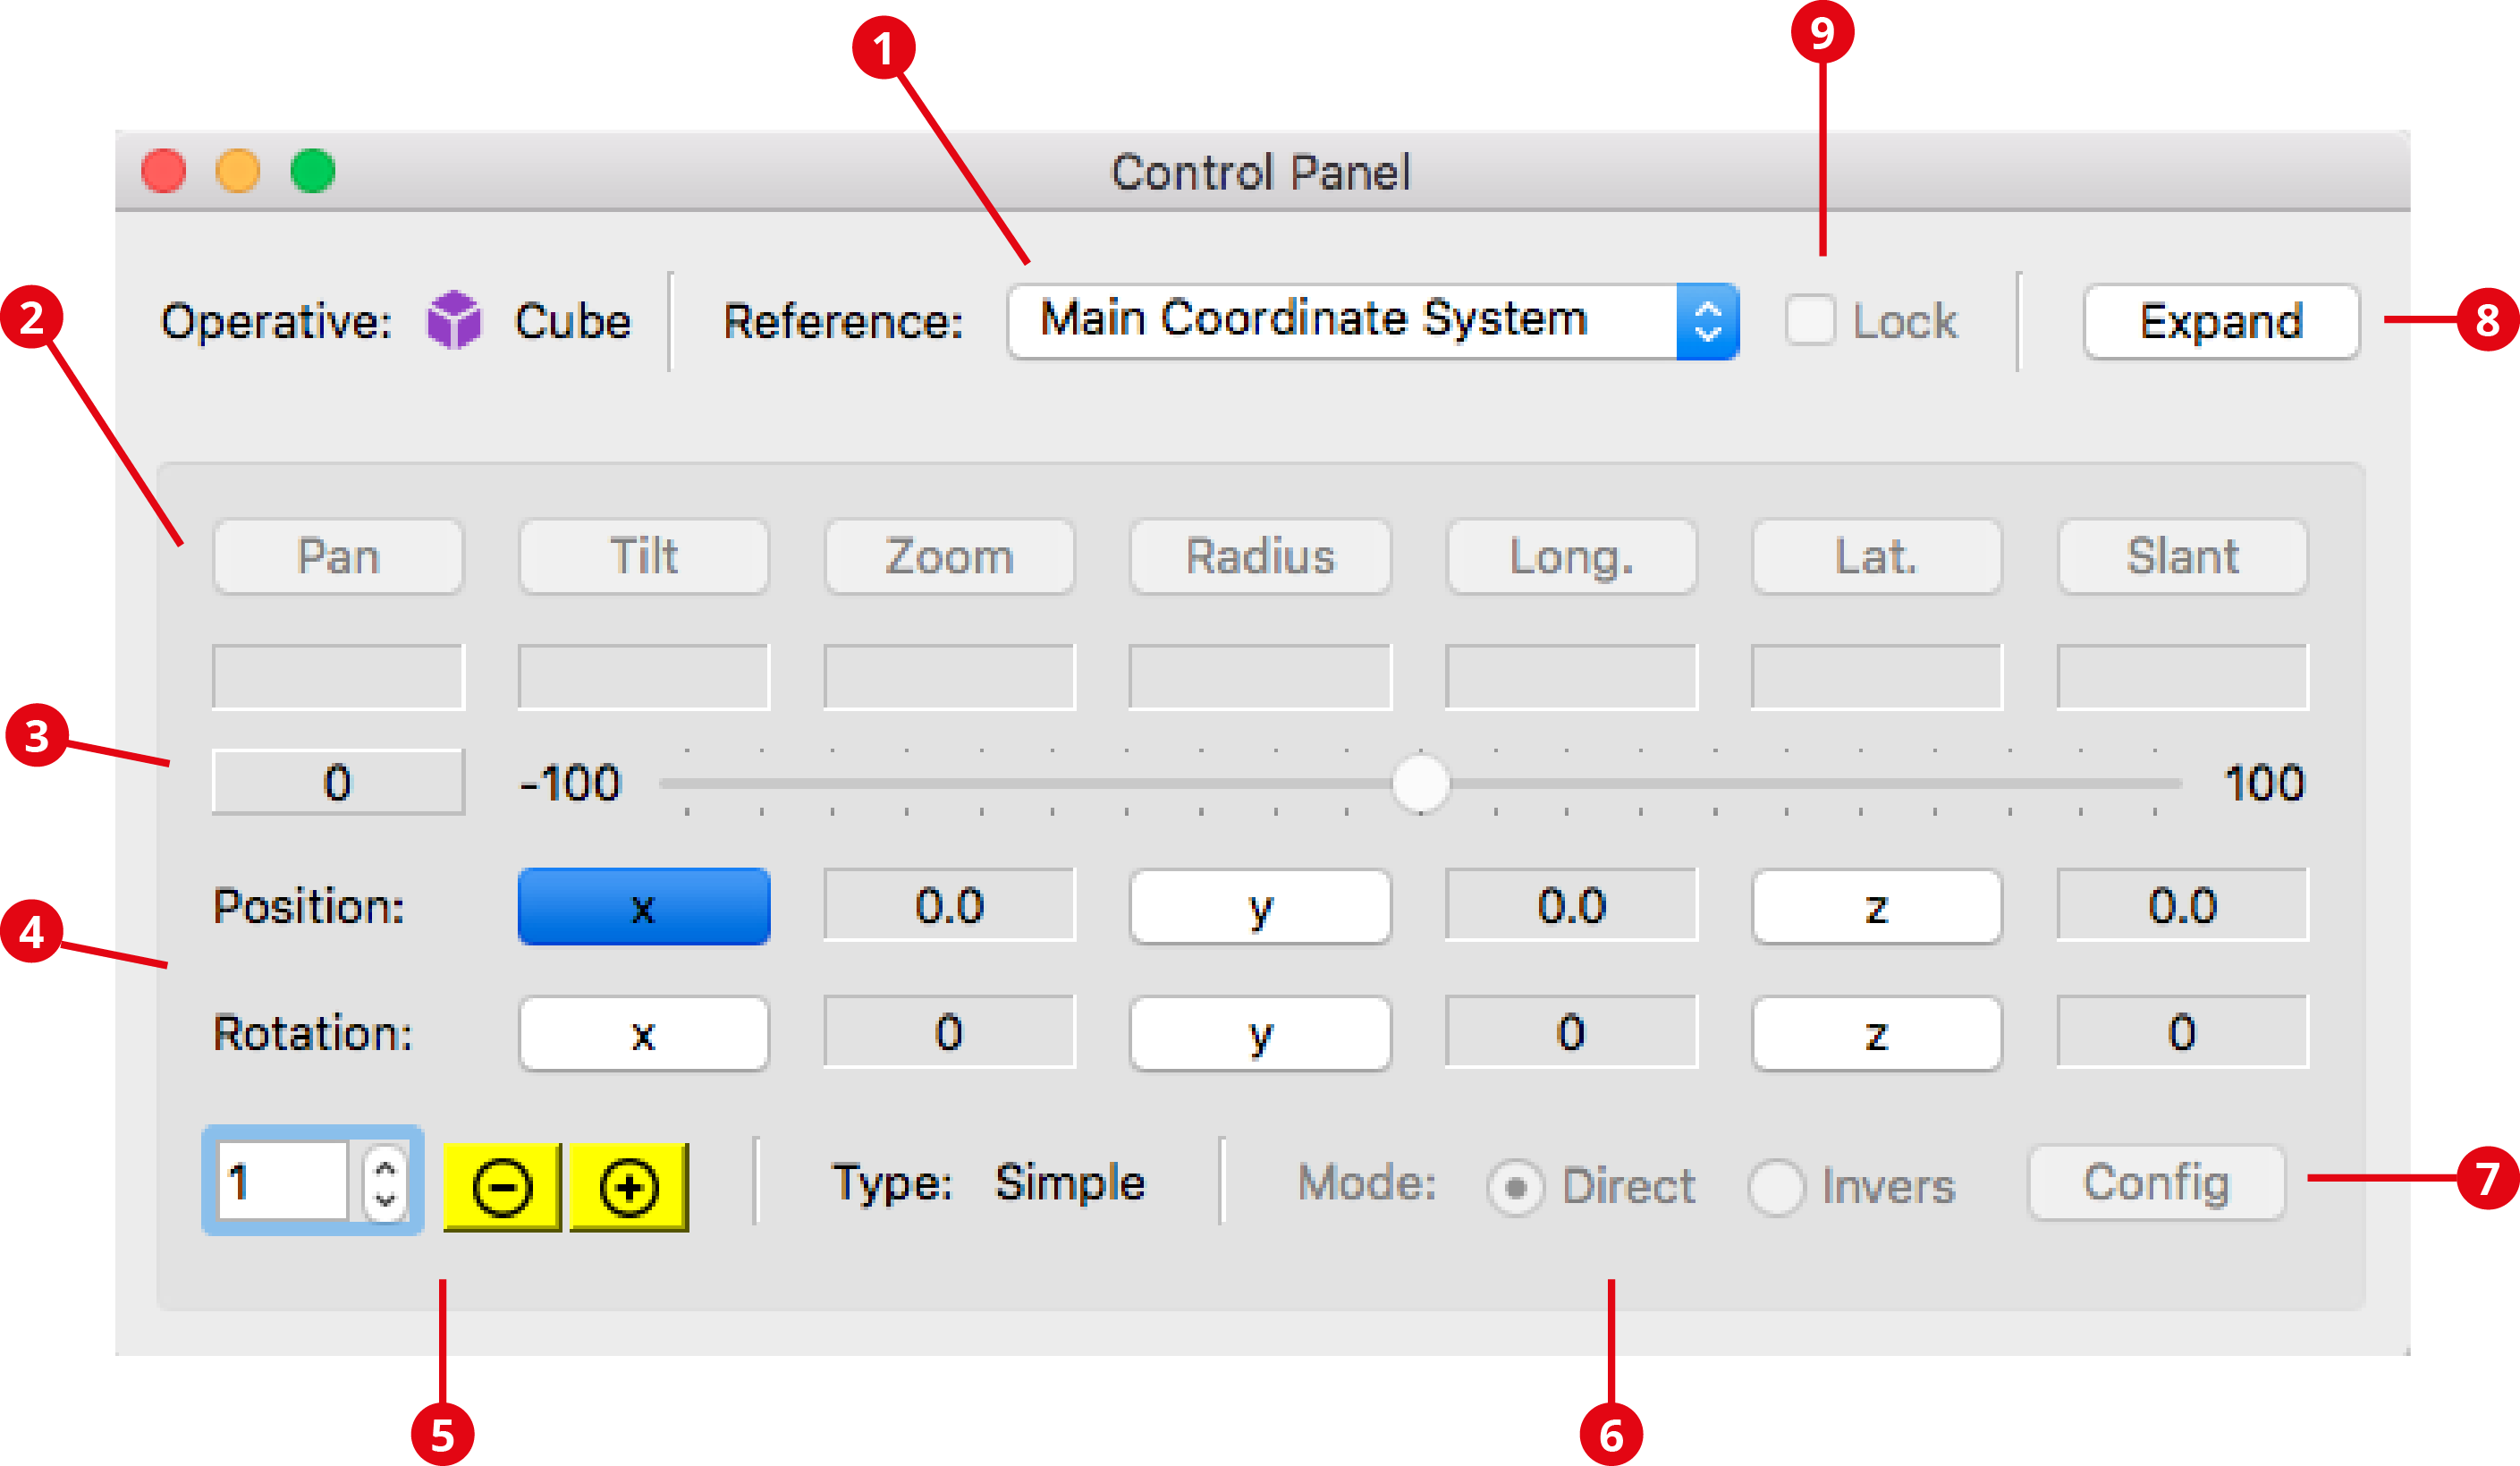
\includegraphics[height=8cm]{images/general_control_nr.png}
    \caption[Control model panel]{Control model panel}
    \label{fig:ctrgeneral}
\end{figure}

The new control GUI for models is presented in \Cref{fig:ctrgeneral}. This interface will look about the same for all models. Some control options are limited depending on the properties of the model. Similarities between this interface and the camera control interface in (figure) can seen. After guidance from the supervisor, the control ability of the camera should be beneficial in use of vehicle and tools for spherical motion. Capacity to move in spherical coordinates opens opportunities for future development of the software. Another significant advantage of this design is that the interface can also substitute the existing control interface for cameras. Based on the old control interface, much improvement had to be done visually and in the underlying code structure. Visualising position and orientation data on the model were something that was missed previously, and regarded as a helpful feature. The values of interest were specified by a method of the supervisor.  It was also aspired to be able to customise button in the form of colour to distinguish the importance functions. One might think that setting another colour on a button would be rather straightforward, but it turns out doing so would reset the stylesheet of that particular button. This means losing the native theme regarding colour and feature properties such as round-corner, size, hovering effect, clicking effect, etc. A simple and effective solution was using an image as the icon for the button. This way the native theme could be kept throughout the different operating systems without setting the properties manually. The GUI have been tested to some extent on a Windows and a Linux operating system. The result so far shows a feasible GUI on both operating systems with no unfortunate design issue. 


A summarise of the functions in the GUI will be presented under, to the number indication in \Cref{fig:ctrgeneral}.
\begin{enumerate}
\item Model movement is related to the chosen reference system. Default on the main coordinate system (world space)
\item Choose of control for movement or rotation in spherical coordinates (in the present not a implemented function and deactivated)

\item Slider control for a smooth and consistent transition (temporarily hard-coded to have an incremental value of 0.1)

\item Choose of control for movement or rotation along the three Cartesian axes.

\item Select incremental value. Increase or decrease by selected value for movement or rotation from the control options in 2. or 4. Remember the last selected value from the associated control options in 2. and 4.

\item Choose to control the model with forward or inverse kinematics. Forward kinematics is selected as default. This function is deactivated for simple models, seen from "Type". The only "complex" type who can use this function, is the serial manipulator model called "robot".

\item Corresponding to 6., only active for the type complex. This function enables the use of the associated control interface followed by the model.

\item Expand the current frame for joystick mode (\Cref{fig:joystick}).

\item Deactivated for the main coordinate system. Enables to lock on other references, such as a path or a model. When locked, the model will move accordingly to the locked reference.
\end{enumerate}

\begin{figure}[ht]
    \centering
    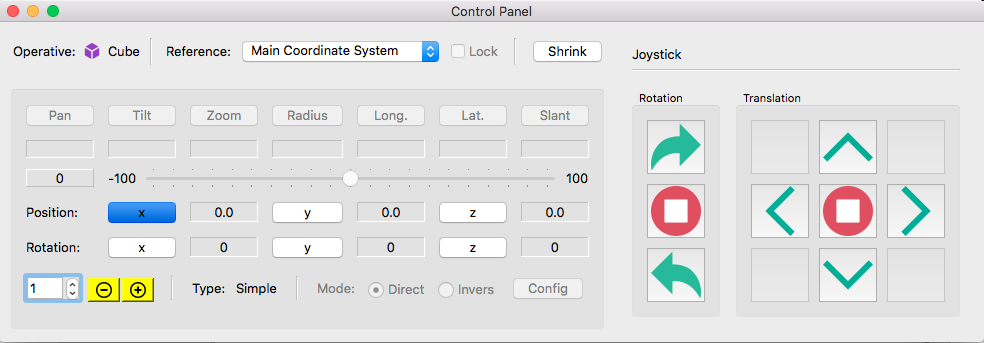
\includegraphics[height=5cm]{images/Joystick.png}
    \caption[Expanded panel for joystick mode]{Expanded panel for joystick mode}
    \label{fig:joystick}
\end{figure}

The expandable panel from \Cref{fig:joystick} was designed as a request to control with the input from a joystick device \cite{joystick}. The GUI for joystick mode is currently a visualise mock-up for future development to utilise and have no functions as of yet.

\section{Frame of reference}

In this implementation of the control system, the connection between the selected model and a chosen reference system had to be developed. The accessible references were based on the basis given from paths, models and the world space. By default, the basis of a model is defined by an offset and an orientation vector relative to the world space. In this case, the frame of reference is the world space. From this, it was reasonably straightforward to change the offset and orientation vector to be relative to the chosen reference of a model space. Adding this function enables a model to switch between references to follow. This allows vehicles and tools to follow given reference system as long it a can be retrieved from the system statically or dynamically. But what if the reference system is not static? The tracked reference system of a vehicle can, for instance, be in motion. A solution to this problem was using the publish-subscribe pattern described in \Cref{chap:pubsub}. This pattern is similar to that of another called Observer pattern \cite{observer_pattern}. But the main difference is that in the observer pattern the sender and the receiver are directly known to each other, which cause dependencies that are not wanted. Another undesirable action is that the receiver is asking the sender if anything has changed. For an autonomous system, adding and removing models dynamically, the publish-subscribe pattern is suitable for this purpose with regards to decoupling \cite{decoupling}. The followed reference system notify if changes occur, those models who are tracking the particular reference will be updated automatically.  

\begin{figure}[ht]
    \centering
    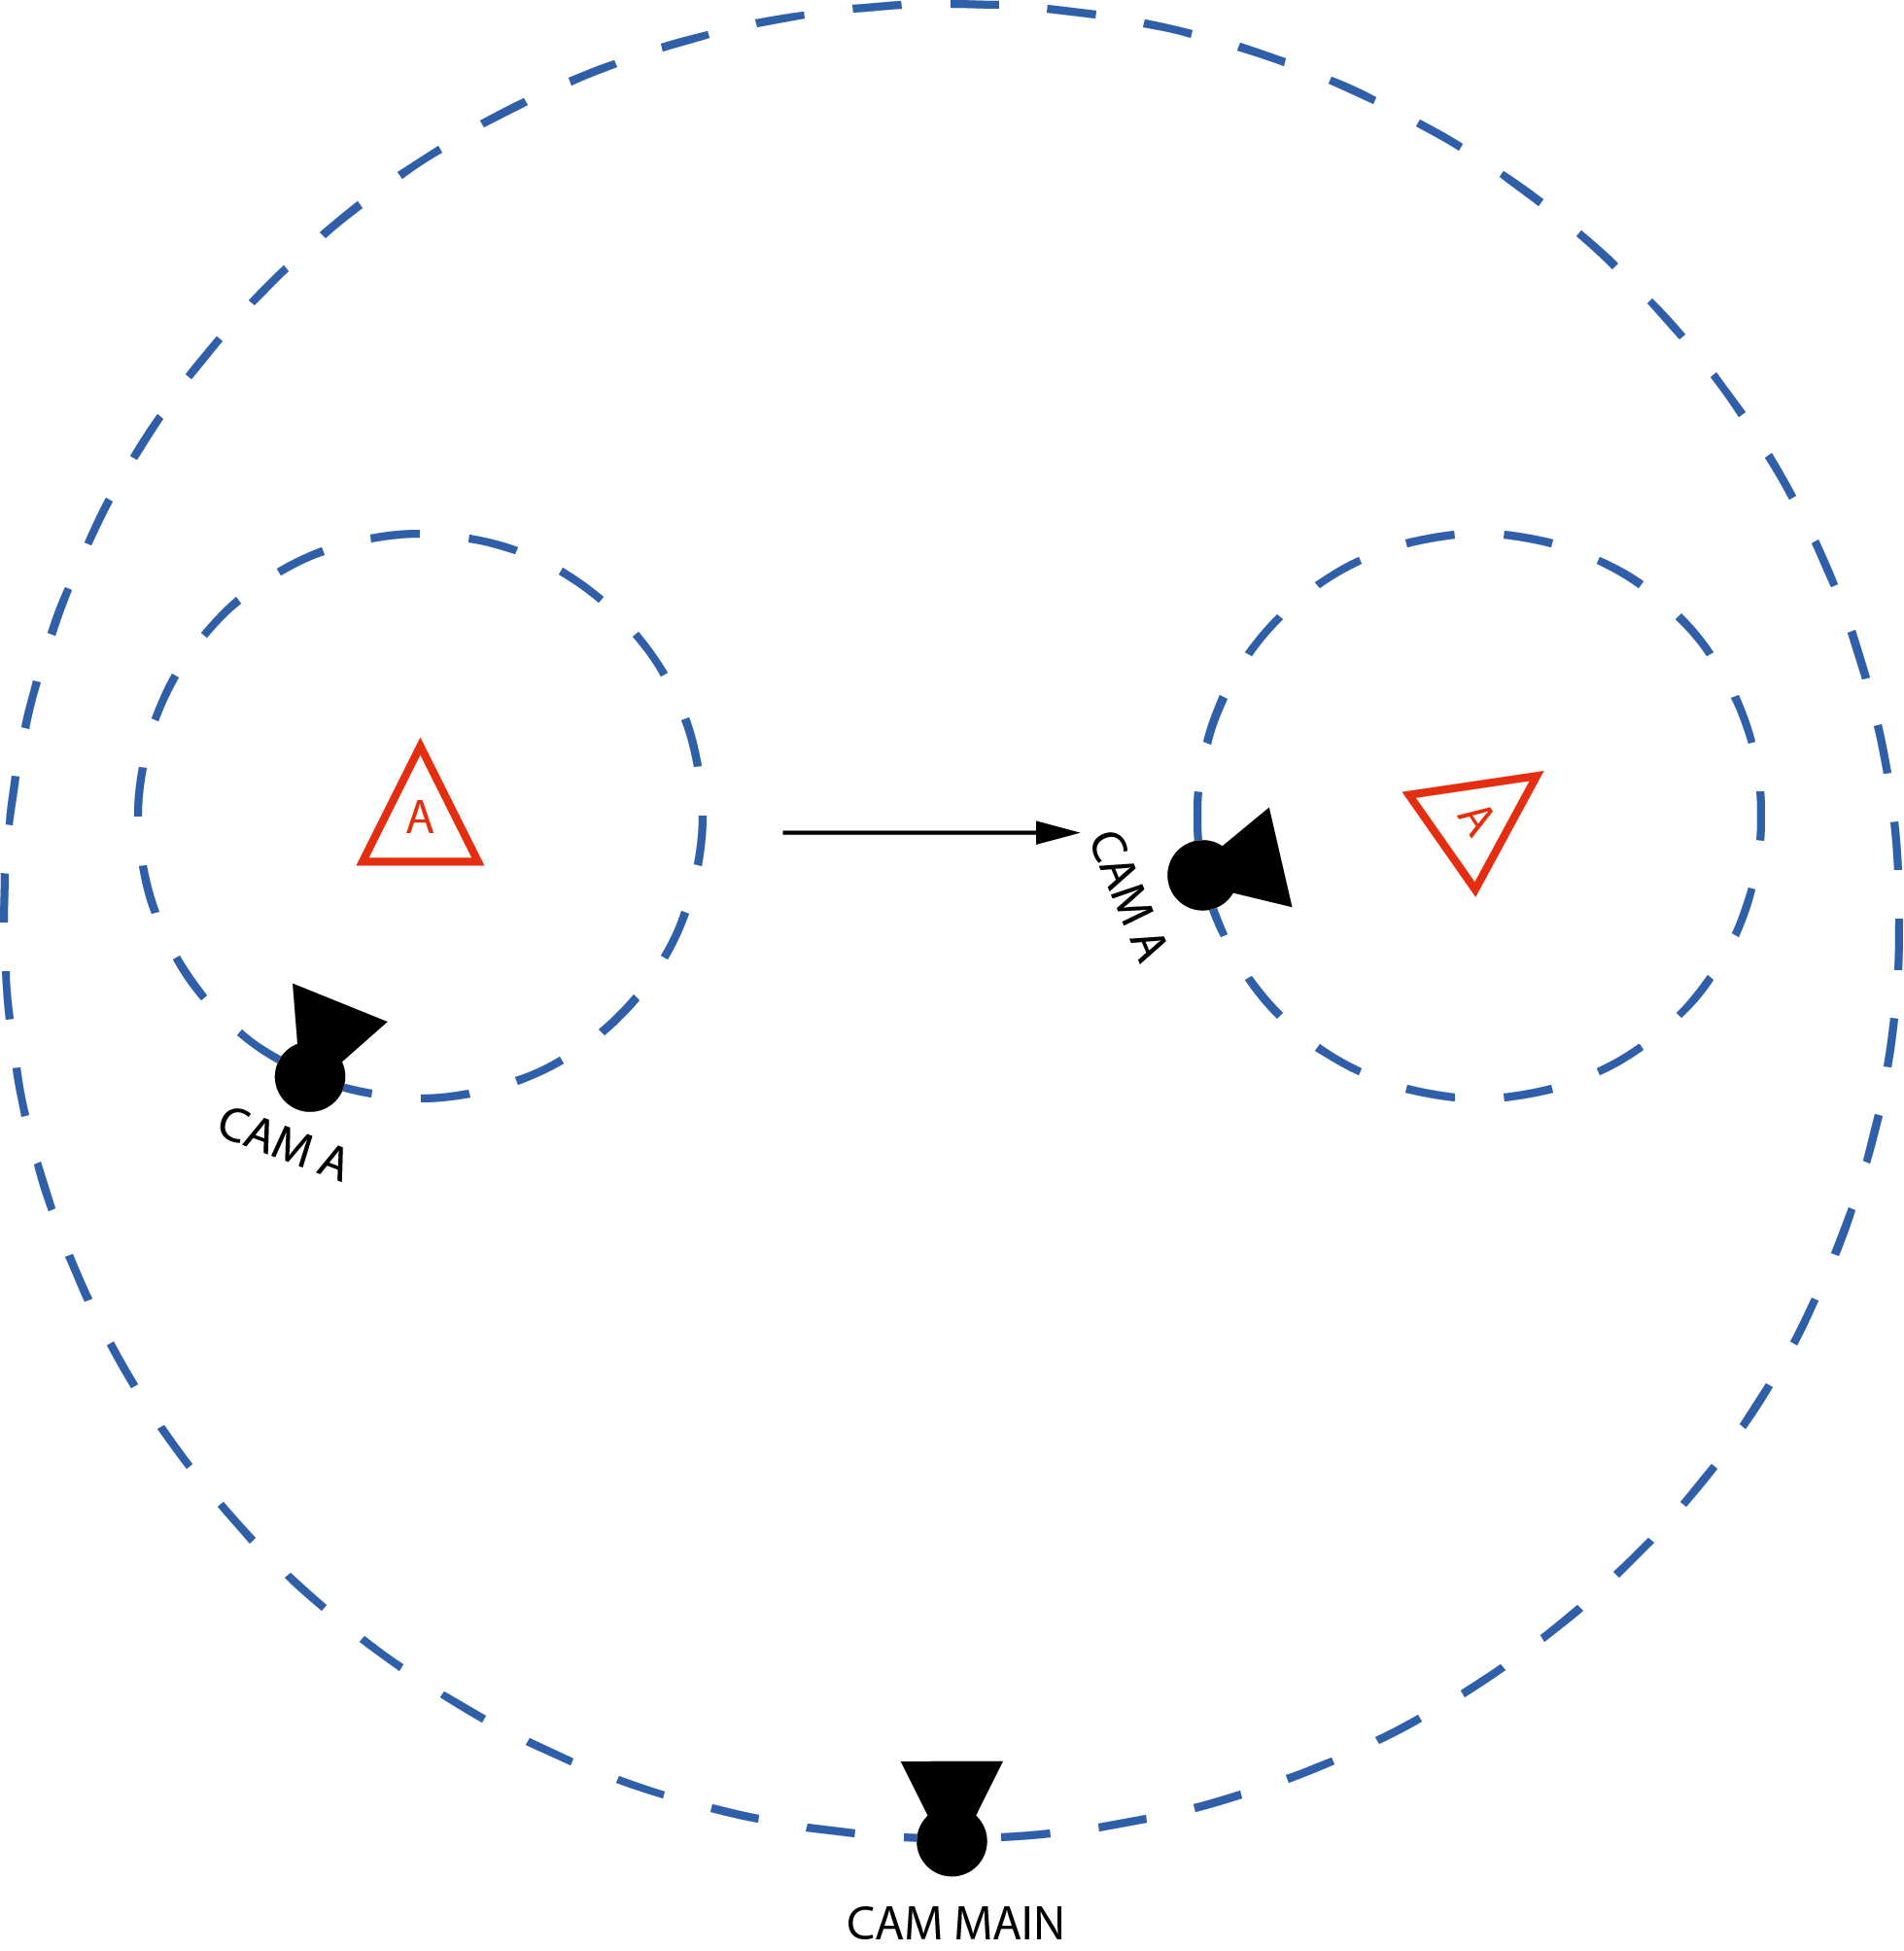
\includegraphics[height=7cm]{images/cam_ex.png}
    \caption[Camera locked on a model]{Camera locked on a model}
    \label{fig:cam_ex}
\end{figure}

This functionality can also be use for cameras and seen as a highly valued feature for future development. The \Cref{fig:cam_ex} illustrate an example for practical usage. In the example, the CAM MAIN is usually the main viewport in the software. CAM A is locked on the model A from a preferred angle, then model A move and rotate to another direction. CAM A is updated with the movement and has kept the same view angle on the model. The viewport can be changed between CAM MAIN and CAM A. This example also show how the system can be used for surveillance of autonomous vehicles. 
\chapter{Controlling Vehicle Tools}

So far, a control system for vehicles has been implemented with a GUI. This chapter will have a look on how to proceed with embedding the control system of the associated tools from a vehicle. Since only one model contains an end-effector, the generalised system will be based on the serial manipulator model (\Cref{fig:SerialManipulator}).

\begin{figure}[ht]
    \centering
    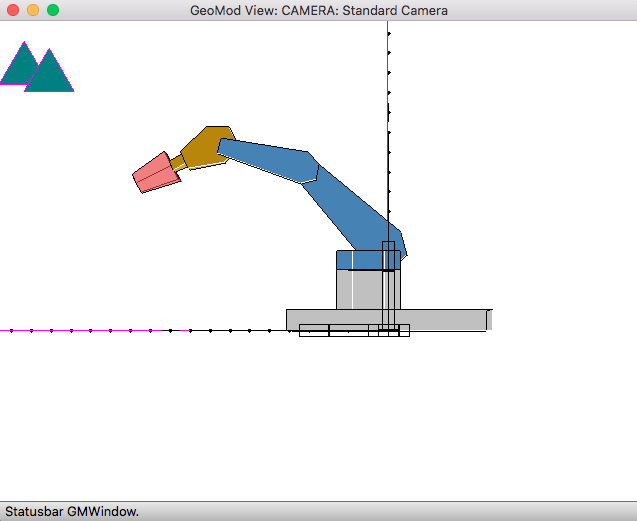
\includegraphics[height=8cm]{images/GeometricModel.png}
    \caption[Geometric model of a serial manipulator]{Geometric model of a serial manipulator.}
    \label{fig:SerialManipulator}
\end{figure}

\section{Kinematics}

It was mentioned that from the work of Martin Lygre Fuglevik, the control system for desired position and orientation of objects along a network of paths was partially implemented. Most of the implementation worked as it should, but some instances regarding rotation in motion to a particular path did not work as prompted. Some small alteration had to be done in the model in order to continue the implementation of the control system. 

\begin{figure}[ht]
    \centering
    \includegraphics[height=7cm]{images/Diagram_Serial_Manipulator.png}
    \caption[Kinematic connection of each part of the serial manipulator model]{Kinematic connection of each part of the serial manipulator model.}
    \label{fig:KinematicsSerialManipulator}
\end{figure}


The \Cref{fig:KinematicsSerialManipulator} illustrates how the communication between each joint is conducted by forward and inverse kinematics on the implemented model. This is done by having variables over the position, rotation and angle on each part of the model. By applying forward kinematics, the joints angle is independently controlled for each parts beginning from the position of the linked mechanism, the base, to the end-effector, i.e. gripper. The function \textit{dirKin()} is an existing implemented function that calculates joint angles of all the joints, when one of the parts is moved. This makes a lot of unnecessary computation considering joints that are not affected by the movements. However, this was neglected as it did not prevent the fulfilment of the current objectives for the project. This should be taken into account in the future for optimisation. 

Forward kinematics works well for a desired end position for the end-effector, but is rather impractical to control when following a path. With inverse kinematics, the position of the base and joint angle is determined from the position of the gripper. Working with inverse kinematics makes it possible to have a desired position for the gripper while the base is under displacement as long as it is within the workspace. Note, it also applies to a displacement of a path. This method of control is very helpful for an AUV, considering currents and other significant disturbances in the ocean. In addition, moving a tool along a path can be achieved, as the joint angles are calculated and set during the series of translation and rotation of the gripper. A control interface for a tool with forward and inverse kinematics can be applied to any model given with a base and an end-effector. 

\begin{figure}[ht]
  \centering
  \subfloat[Forward kinematics]{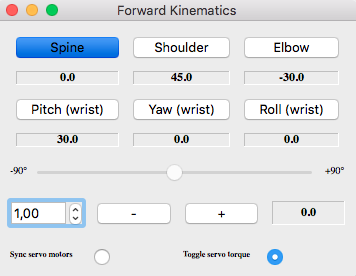
\includegraphics[width=0.31\textwidth]{images/forward.png}\label{fig:forward}}
  \hfill
  \subfloat[Inverse kinematics]{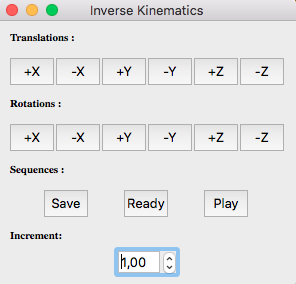
\includegraphics[width=0.31\textwidth]{images/inverse.png}\label{fig:inverse}}
  \hfill
  \subfloat[Motion control]{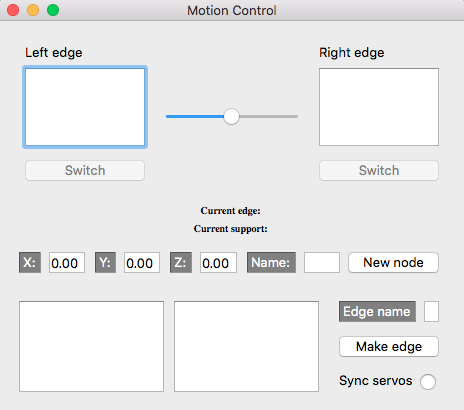
\includegraphics[width=0.31\textwidth]{images/Motion.png}\label{fig:motion}}
  \caption[Control panels implemented by Martin Lygre Furevik]{Control panels implemented by Martin Lygre Furevik.}
  \label{fig:martincontrolpanels}
\end{figure}

The implementation of the inverse kinematics solver for this specific model was developed by Professor Sven Fjeldaas \cite{sven}. In Martin Lygre Fureviks' master thesis, the inverse kinematics solver was implemented in the model with a corresponding control panel for the inverse kinematics. A similar control panel for forward kinematics was also made for the model. Furthermore, a motion controller for the robot was created to move the gripper along a path. The controls for the forward, inverse kinematics and motion can be seen in \Cref{fig:martincontrolpanels}. The implementation of the motion controller is flexible and generalised, requiring only a tool and a path to work. This is done by connecting a pointer to the tool variable from an end-effector model, like the gripper, and a pointer to the path variables from a model. Any given model can, therefore, be freely moved along a given path. For tools, the motion on the path calls the inverse kinematics implemented in the model to regulate the relation between the vehicle and the tool. Combining the motion controller with the implemented control system for this project, tracking a path while the base or the path is in motion is now possible to demonstrate in GeoMod (\Cref{fig:displacement}). 


\begin{figure}[ht]
  \centering
  \subfloat[The gripper is following a path.]{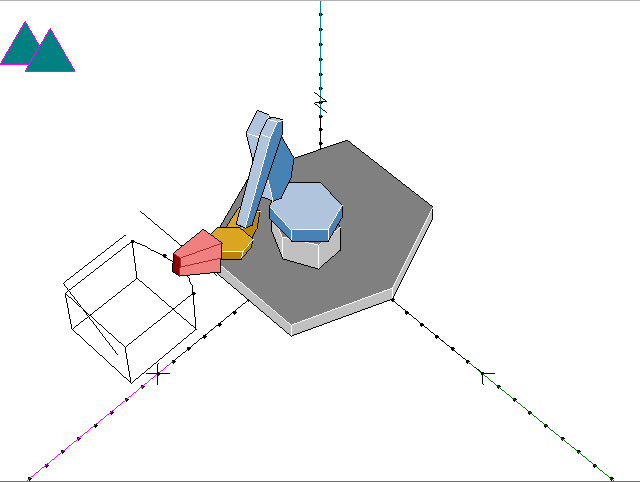
\includegraphics[width=0.4\textwidth]{images/serial_1.png}\label{fig:s1}}
  \hfill
  \subfloat[The gripper is still following the path, during displacement.]{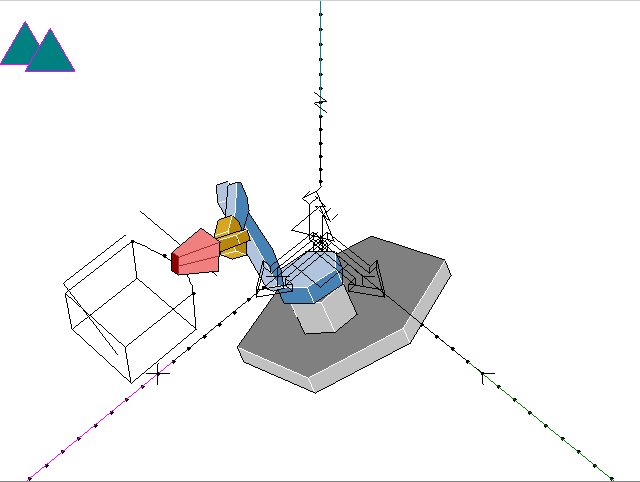
\includegraphics[width=0.4\textwidth]{images/serial_2.png}\label{fig:s2}}
  \caption[Displacement of the base of the serial manipulator model]{Displacement of the base of the serial manipulator model.}
  \label{fig:displacement}
\end{figure}
%\chapter{Discussion}

\section{Further Work}



\chapter{Conclusion}

\section{Result}
An interactive GUI for the control system has been implemented. The method uses different modules to achieve a working control system for vehicles and tools, represented as geometrical models. It has been made to adapt to models that are dynamically linked to the library in GeoMod. This has been done under consideration for an autonomous mode employed by other systems. 

The designed GUI enables control over position and orientation of a model in a three-dimensional space. It is arranged such that translation and rotation can be done along the three Cartesian axes and with the possibility for spherical motion in future development. Options to move relative to a chosen reference system has been implemented. This allows models and tools to follow the corresponding reference, existing or added, in GeoMod. Value information in the form of their respective coordinate system is displayed as useful instruments. The transition of movement is no longer predetermined as it is now possible to configure displacement to all directions. Controlling model represented as a vehicle with a tool, enables control choices for forward and inverse kinematics. The implemented control system supports interaction between models and tracking path with or without a tool.

\section{Discussion}

Much of the functionality had to be revised to create a working control system. A major challenge was to solve how the data needed was passed between different modules, as the implementations originally were done independently. As more module and functionality is added, the increase of connection and interactions gets more complicated to handle for a working control system. Finally, a GUI that emphasises the structure, intuitiveness and a compact design had to be kept in mind for the user to utilise. The GUI is arranged such that new features can be implemented, and also further develop awaited functions needed. Some of these functionality has been mentioned throughout this project, e.g. spherical translation, joystick input and appropriate interface for cameras. The control system for tools was to some degree implemented in the control systems. To base this system simply on one single model with corresponding tool, limits the feasibility of testing and assumption for developing a functional control system. A generalised GUI primarily for tools with the use of forward and inverse kinematics was not developed under this project. However, the framework and the approach has been reviewed during this project to serve as a foundation for further implementation in the future.

The successfulness of this assignment can be assessed on the basis of how the proceeded and achieved efforts have resolved or contributed to the objectives in \cref{chap:objectives}. With the newly implemented control system, the project has made some progress towards a unified system that is suited to test and demonstrate autonomous interactions of vehicles and tools.

% Bibliography - edit references.bib and use the \cite command in text
\renewcommand{\bibname}{References}
\bibliographystyle{plain}
\bibliography{references}

%\addcontentsline{toc}{chapter}{\bibname}

\clearpage
\clearpage
\vspace*{\fill}
{\centering\huge\bfseries Appendix \par}
\vspace*{\fill}

\phantomsection
\addcontentsline{toc}{chapter}{Appendix}

\addcontentsline{toc}{chapter}{A Project Assignment}


\addcontentsline{toc}{chapter}{B Formal Project requirement}


\addcontentsline{toc}{chapter}{C Risk Assessment}

%\pagenumbering{arabic}% resets `page` counter to 1
%\renewcommand*{\thepage}{A-\arabic{page}}


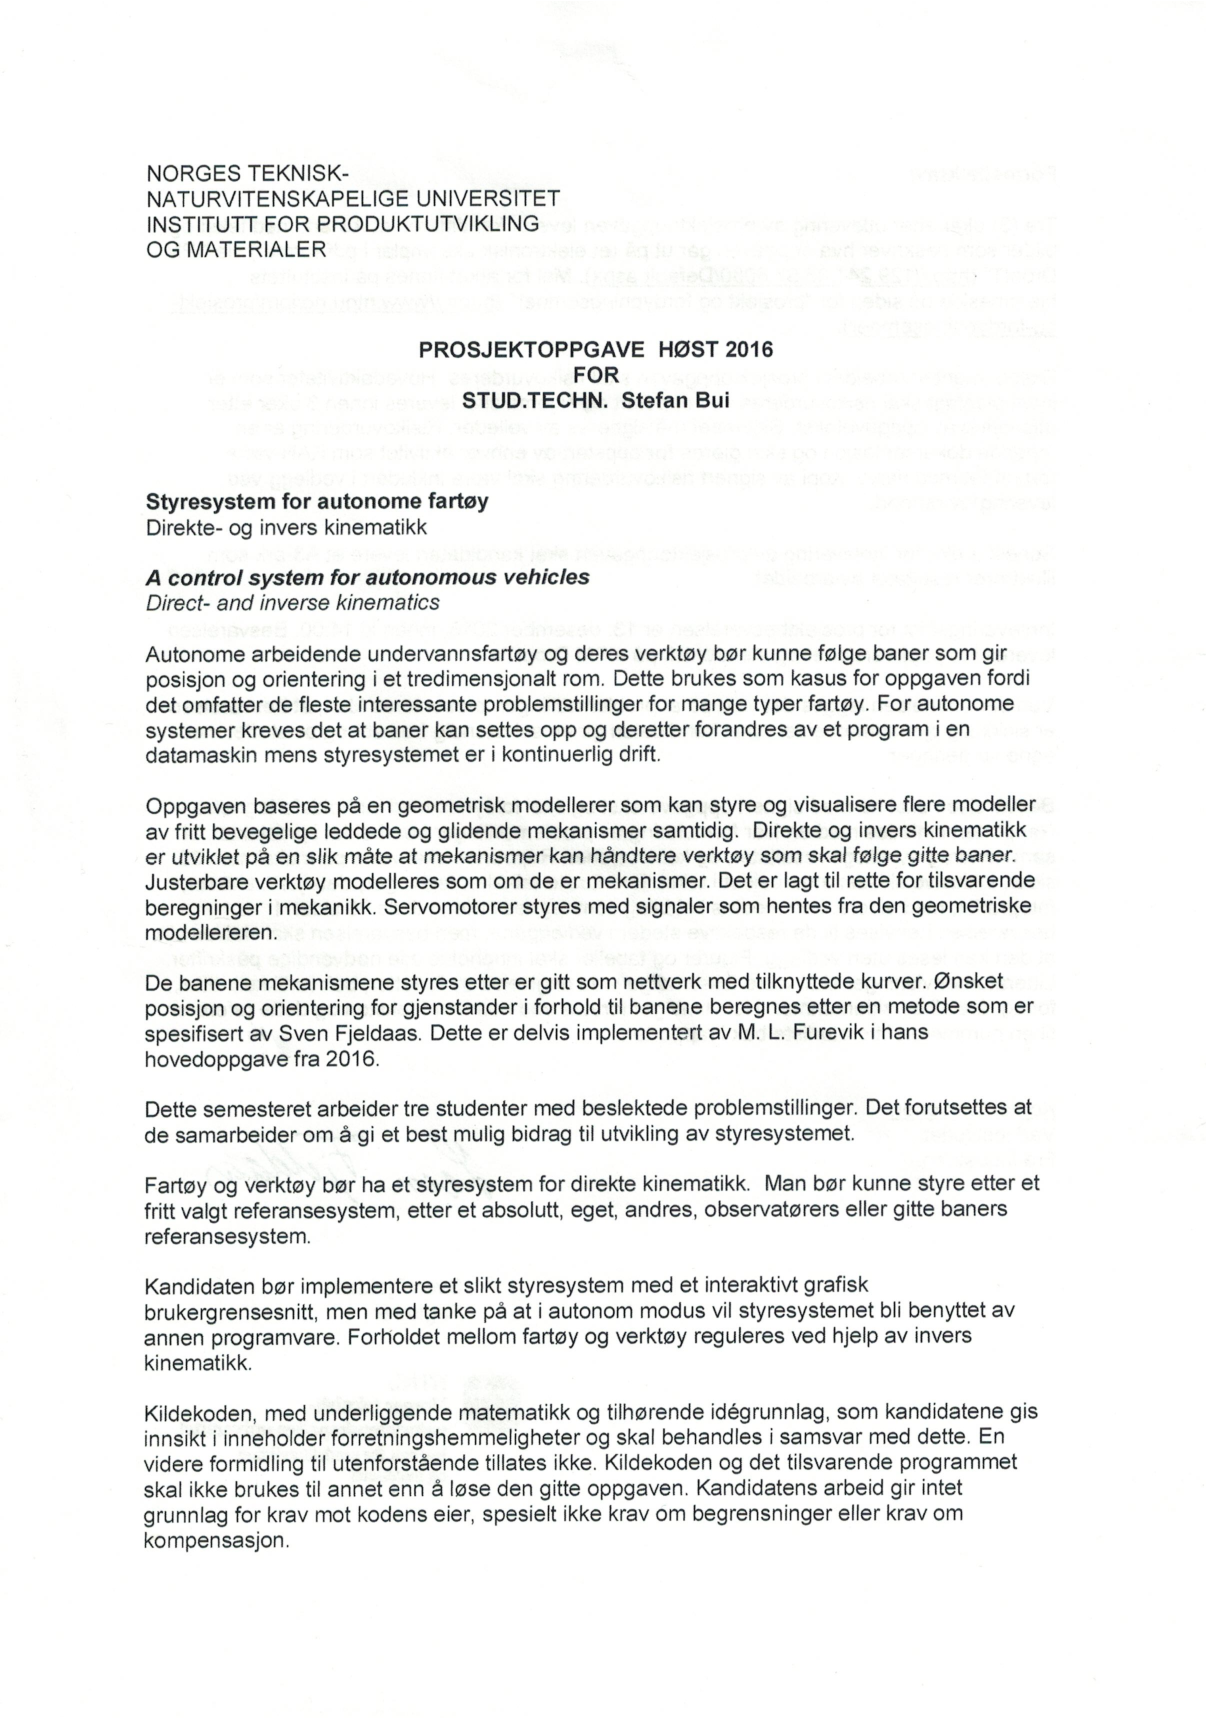
\includepdf[pages=-]{appendix/pdf/assignment.pdf}

\includepdf[pages=2]{appendix/pdf/assignment.pdf}
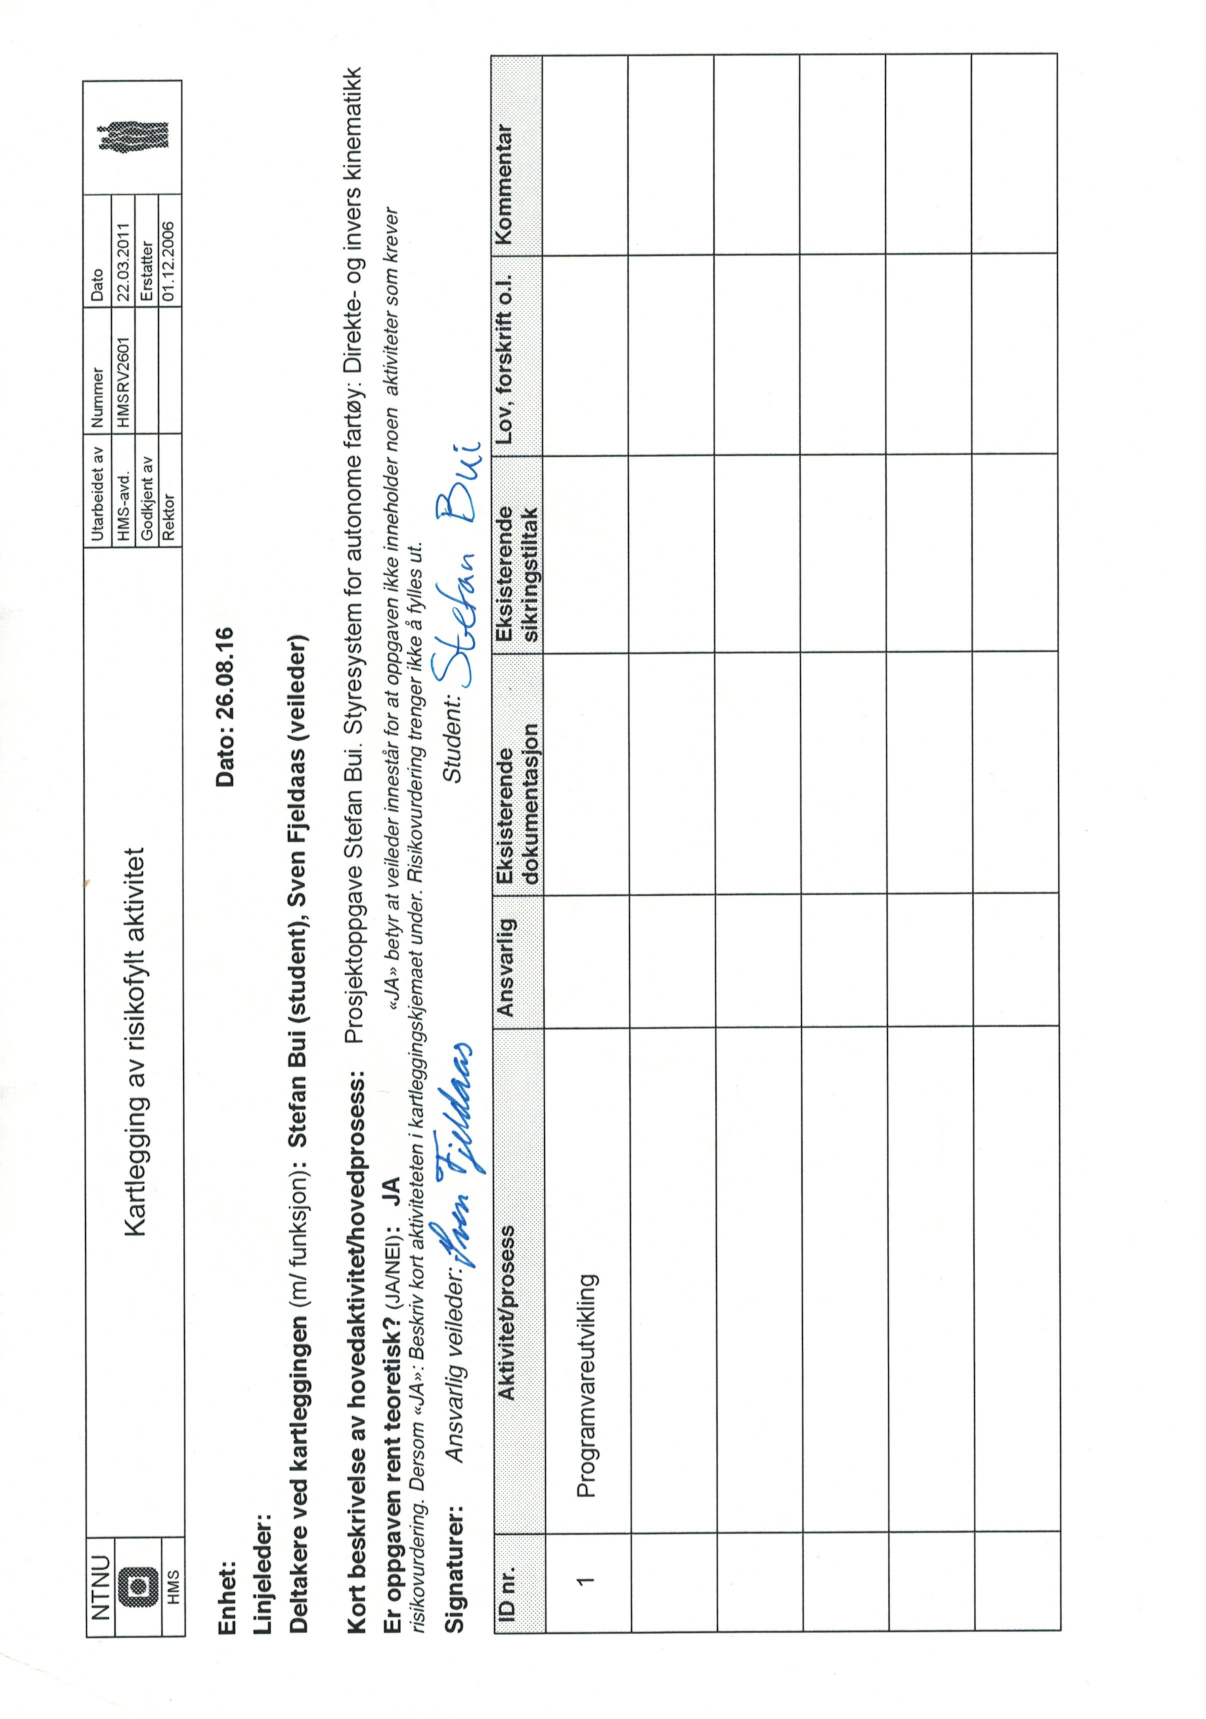
\includepdf[pages=-]{appendix/pdf/risk.pdf}


\end{document}
